\chapter{Theoretische Grundlagen}
\thispagestyle{fancy}
\textbf{Hier fehlt noch eine generelle Einleitung zum Kapitel}

\section{Struktur der Anwendung}
In diesem Abschnitt soll zunächst die generelle Struktur der Anwendung definiert werden. Weite Teile der Struktur können dabei aus dem Praxisprojekt übernommen werden. Im Praxisprojekt wurden die folgenden Themengebiete behandelt:

\begin{itemize}
  \item Typographie
  \item Layout \& Struktur
  \item Whitespace
  \item Farben
  \item Bilder
  \item Interaktive Elemente
\end{itemize}

Nach einer erneuten evaluation der Ergebnisse des Praxisprojektes konnten die in der Abschlussarbeit zu behandelnden Themengebiete auf zunächst drei eingegrenzt werden (der Bereich \textit{Layout \& Struktur} wurde dabei in \textit{Layout \& Grids} umbenannt):

\begin{itemize}
  \item Typographie
  \item Layout \& Grids
  \item Farben
\end{itemize}

Diese Abgrenzung begründet sich auf verschiedene Weisen. Im Fall des Bereiches \textit{Whitespace} konnte im Rahmen des Praxisprojektes kein zufriedenstellendes Konzept erarbeitet werden, wodurch sich dieser Bereich per se nicht für eine Umsetzung eignet. Weiterhin muss es Ziel dieser Arbeit sein, am Schluss eine vollständige Anwendung zu erhalten. Um dieses Ziel im zeitlichen Rahmen erreichen zu können mussten weitere Themengebiete vernachlässigt werden. Hier boten sich die Bereiche \textit{Bilder} und \textit{Interaktive Elemente} an, da diese für die gestalterische Grundqualität eine vergleichsweise niedrige Rolle spielen. \textbf{NOTE: Vielleicht muss das hier noch belegt werden, wie ein Brötchen}. Diese Bereiche wurden aber ausreichend konzeptioniert und bieten sich als erste Erweiterungen für die Anwendung nach beenden der Arbeit an.

Außerdem müssen für die Anwendung jeweils ein nutzerfreundlicher Einstieg und Ausstieg gefunden werden. Diese wurden im Praxisprojekt nicht explizit ausgearbeitet und fallen somit auch Konzeptionell in den Bereich der Abschlussarbeit und werden später in diesem Kapitel behandelt.

Die finale Struktur der Anwendung für den Rahmen dieser Arbeit sieht also wie folgt aus:

\begin{itemize}
  \item Einstieg
  \item Typographie
  \item Layout \& Grids
  \item Farben
  \item Ausstieg
\end{itemize}

\subsection{Einstieg in die Anwendung}
Bereits im Praxisprojekt wurde festgestellt, dass es sinnvoll ist, das Zielmedium des Nutzers zu kennen. Mit Blick auf die Zielgruppe wurden hier drei mögliche Bereiche definiert: Native App, Website und Textdokument. \textbf{NOTE: Hier verweis auf Untersuchung im PP}. Diese Bereiche können jedoch auch in sich verschiedene Eigenarten aufweisen, so kann ein Textdokument beispielsweise für das Lesen an einem Bildschirm oder das Lesen in gedruckter Form entworfen werden. Eine komplette Auflistung der möglichen Bereiche oder \textit{scopes} der Anwendung findet sich in Abbildung \ref{fig:intro} auf Seite \pageref{fig:intro}.

\begin{figure}[h]
    \centering
    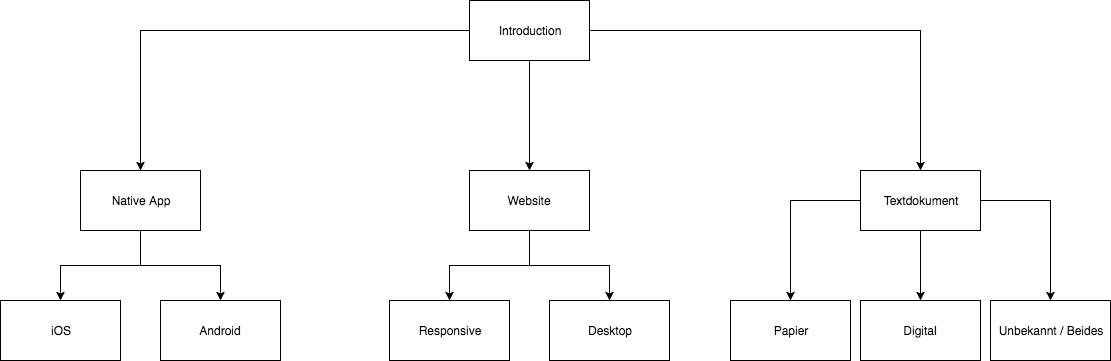
\includegraphics[width=1\textwidth]{images/ablauf_intro.png}
    \caption{Mögliche Entscheidungen im Einstieg der Anwendung}
    \label{fig:intro}
\end{figure}

Obwohl die Abgrenzung der Bereiche für die hier definierte Zielgruppe ausreichend ist, lassen sich bereits jetzt einige Stellen erkennen, die bei einer möglichen späteren Erweiterung der Zielgruppe überarbeitet werden müsste. Vorrangig betrifft das den Bereich \textit{Website}. Hier ist die vorhandene Unterteilung in \textit{Responnsive} und \textit{Desktop} für ein Echtwelt-Szenario unter Umständen zu allgemein gehalten.

Um den kognitiven Aufwand \textbf{Beleg} für den Nutzer möglichst gering zu halten, bietet es sich an, ihn Schrittweise durch das Festlegen des für ihn passenden Bereiches zu führen.

\subsection{Ergebnisse der Benutzung}
Bei der Textgestaltung und automatischen Änderung von Abbildungsnummern, Querverweisen,
Seitenzahlen, Gliederungen, Literaturhinweisen etc. bietet sich der Rückgriff
auf moderne Textverarbeitungsprogramme an. Nutzen Sie diese zur besseren Lesbarkeit
und Strukturierung des Textes, aber vermeiden Sie überflüssige Spielereien. Da
besonders bei Textdokumenten mit eingebundenen Objekten wie Bildern, Formeln

\section{Diskussion verfügbarer Technologien}
Bei der Textgestaltung und automatischen Änderung von Abbildungsnummern, Querverweisen,
Seitenzahlen, Gliederungen, Literaturhinweisen etc. bietet sich der Rückgriff
auf moderne Textverarbeitungsprogramme an. Nutzen Sie diese zur besseren Lesbarkeit
und Strukturierung des Textes, aber vermeiden Sie überflüssige Spielereien. Da
besonders bei Textdokumenten mit eingebundenen Objekten wie Bildern, Formeln

\subsection{Vue.js}
Bei der Textgestaltung und automatischen Änderung von Abbildungsnummern, Querverweisen,
Seitenzahlen, Gliederungen, Literaturhinweisen etc. bietet sich der Rückgriff
auf moderne Textverarbeitungsprogramme an. Nutzen Sie diese zur besseren Lesbarkeit
und Strukturierung des Textes, aber vermeiden Sie überflüssige Spielereien. Da
besonders bei Textdokumenten mit eingebundenen Objekten wie Bildern, Formeln

\subsection{Angular.js}
Bei der Textgestaltung und automatischen Änderung von Abbildungsnummern, Querverweisen,
Seitenzahlen, Gliederungen, Literaturhinweisen etc. bietet sich der Rückgriff
auf moderne Textverarbeitungsprogramme an. Nutzen Sie diese zur besseren Lesbarkeit
und Strukturierung des Textes, aber vermeiden Sie überflüssige Spielereien. Da
besonders bei Textdokumenten mit eingebundenen Objekten wie Bildern, Formeln

\subsection{React.js}
Bei der Textgestaltung und automatischen Änderung von Abbildungsnummern, Querverweisen,
Seitenzahlen, Gliederungen, Literaturhinweisen etc. bietet sich der Rückgriff
auf moderne Textverarbeitungsprogramme an. Nutzen Sie diese zur besseren Lesbarkeit
und Strukturierung des Textes, aber vermeiden Sie überflüssige Spielereien. Da
besonders bei Textdokumenten mit eingebundenen Objekten wie Bildern, Formeln

\section{Technologie-Stack}
Bei der Textgestaltung und automatischen Änderung von Abbildungsnummern, Querverweisen,
Seitenzahlen, Gliederungen, Literaturhinweisen etc. bietet sich der Rückgriff
auf moderne Textverarbeitungsprogramme an. Nutzen Sie diese zur besseren Lesbarkeit
und Strukturierung des Textes, aber vermeiden Sie überflüssige Spielereien. Da
besonders bei Textdokumenten mit eingebundenen Objekten wie Bildern, Formeln

\section{Gestaltung}
Bei der Textgestaltung und automatischen Änderung von Abbildungsnummern, Querverweisen,
Seitenzahlen, Gliederungen, Literaturhinweisen etc. bietet sich der Rückgriff
auf moderne Textverarbeitungsprogramme an. Nutzen Sie diese zur besseren Lesbarkeit
und Strukturierung des Textes, aber vermeiden Sie überflüssige Spielereien. Da
besonders bei Textdokumenten mit eingebundenen Objekten wie Bildern, Formeln
